
\newpage
\section{Chapter 1 - Probability}

\subsection*{Exercises}

%%%%%%%%%%%%%%%%%%%%%%%%%%%%%%%%%%%%%%%%%%%%%%%%%%%%%%%%%%%%%%%%%%%%%%%%%%%%%%%
\textbf{1.1}\\  % PDF page 13
Proving the Continuity of Probabilities.

\bigskip\noindent
\textbf{1.8 Theorem} (Continuity of Probabilities). If $A_n\rightarrow A$
then
\[
    \P(A_n)\rightarrow\P(A)
\]
as $n\rightarrow\infty$.

\bigskip\noindent
\textsc{Proof}. Suppose that $A_n$ is monotone increasing so that
$A_1\subset A_2 \subset\ldots$.
Let $A = \lim_{n\ra\infty} A_n = \bigcup_{i=1}^\infty A_i$.
Define:
\begin{align*}
    B_1 &= A_1 \\
    B_2 &= \{\omega\in\Omega \;:\; \omega\in A_2,\omega\not\in A_1\} \\
    B_3 &= \{\omega\in\Omega \;:\; \omega\in A_3,\omega\not\in A_2,\omega\not\in A_1\} \\
    \vdots &
\end{align*}
\textbf{(1)} Showing that $B_i$ are disjoint sets.\\
We have $B_1 = A_1$. Since $B_2 = \{\omega\in\Omega \;:\; \omega\in A_2,\omega\not\in A_1\}$,
we can rewrite this as $B_2 = A_2 - A_1$ by definition of set difference.

Since $B_3 = \{\omega\in\Omega \;:\; \omega\in A_3,\omega\not\in A_2,\omega\not\in A_1\}$
and since $A_1\subset A_2$, we can rewrite this as $B_3 = A_3 - (A_1\bigcup A_2)$.
In general; $B_k = A_k - (\bigcup_{i=1}^{k-1}A_i)$.

Assuming some random sets $B_m$, $B_p$ for some $m,p\in\N$. Without loss of generality,
we assume $m > p$. Then:
\begin{align*}
    B_m\bigcap B_p &=
    \Big(A_m - (\bigcup_{i=1}^{m-1}A_i)\Big)\bigcap \Big(A_p - (\bigcup_{i=1}^{p-1}A_i)\Big)\\
    &= 
    \Big(A_m \bigcap(\bigcup_{i=1}^{m-1}A_i)^c\Big)\bigcap \Big(A_p \bigcap (\bigcup_{i=1}^{p-1}A_i)^c\Big)\\
    \shortintertext{DeMorgan's law}
    &= 
    \Big(A_m \cap A_1^c \cap A_2^c \cap \ldots \cap A_p^c \cap \ldots \cap A_{m-1}^c\Big)\bigcap
    \Big(A_p \cap A_1^c \cap A_2^c \cap \ldots \cap A_{p-1}^c\Big) \\
\shortintertext{Reshuffling terms and repeated use of $C\cap C = C$}
    &= A_m \cap A_1^c \cap A_2^c \cap \ldots \cap \underbrace{A_p^c\cap A_p}_{=\emptyset} \cap \ldots \cap A_{m-1}^c\Big) \\
    &= \emptyset
\end{align*}
Since $B_m\cap B_p = \emptyset$, they are disjoint. (\emph{Quite certain this is a correct argument, but could have
made it a bit easier by going directly to the $A_3\cap A_2^c\cap A_1^c$ version of the sets.})


\medskip\noindent
\textbf{(2)} Showing that 
\[
A_n = \bigcup_{i=1}^n A_i = \bigcup_{i=1}^n B_i
\]
for each $n$. Showing this with an induction argument. Note that $A_1 = B_1$, and $A_2\cup A_1 = A_2$ since $A_1\subset A_2$. Note also that:
\begin{align*}
    B_2\cup B_1 &= (A_2\cap A_1^c)\cup A_1 \\
    &= (A_2\cup A_1)\cap(A_1^c\cup A_1) \\
    &= (A_2\cup A_1)\cap(\Omega) \\
    &= A_2\cup A_1 \\
    &= A_2
\end{align*}
So this is true for $n=2$. Assume that $A_k = \cup_{i=1}^k A_i = \cup_{i=1}^k B_i$ for $k\in\N$. Showing that this applies to $k+1$.
$$
\bigcup_{i=1}^{k+1} A_i = A_{k+1}\cup\Big(\bigcup_{i=1}^{k}A_i\Big) = A_{k+1}\cup A_k = A_{k+1}
$$
\begin{align*}
    \bigcup_{i=1}^{k+1} B_i &= B_{k+1}\cup\Big(\bigcup_{i=1}^{k} B_i\Big)\\
    &= B_{k+1}\cup A_k \\
    &= \Big[A_{k+1}\cap \Big(A_k^c\cap\ldots\cap A_1^c\Big)\Big]\cup A_k \\
    &= \Big[A_{k+1}\cap \Big(A_k\cup\ldots\cup A_1\Big)^c\Big]\cup A_k \\
    %\shortintertext{Since $A_j\subset A_{j+1}$.}
    &= \Big[A_{k+1}\cap A_k^c\Big]\cup A_k \\
    &= (A_{k+1}\cup A_k)\cap (A_k^c\cup A_k) \\
    &= (A_{k+1}\cup A_k)\cap\Omega \\
    &= A_{k+1}\cup A_k \\
    &= A_{k+1}
\end{align*}
Result verified by induction argument.

\medskip\noindent
\textbf{(3)} Showing that 
\[
\bigcup_{i=1}^\infty B_i = \bigcup_{i=1}^\infty A_i.
\tag{$\diamondsuit$}
\]
By definition:
$$
A = \lim_{n\ra\infty} A_n = \bigcup_{i=1}^\infty A_i.
$$
By step (2):
$$
A = \lim_{n\ra\infty} A_n = \lim_{n\ra\infty}\bigcup_{i=1}^n A_i = \lim_{n\ra\infty}\bigcup_{i=1}^n B_i = \bigcup_{i=1}^\infty B_i.
$$
Hence, $(\diamondsuit)$ is satisfied.

\newpage\noindent
%%%%%%%%%%%%%%%%%%%%%%%%%%%%%%%%%%%%%%%%%%%%%%%%%%%%%%%%%%%%%%%%%%%%%%%%%%%%%%%
\textbf{1.2}\\  % PDF page 13
Proving some well known results by using the axioms:
\begin{align*}
    \P(A) \geq 0,\;\forall A\subset\Omega \tag{A.1} \\
    \P(\Omega) = 1, \tag{A.2} \\
    \P\left(\bigcup_{i=1}^\infty A_i\right) = \sum_{i=1}^\infty \P(A_i) \tag{A.3}
\end{align*}
where $A_1, A_2,\ldots$ are disjoint in  $(A.3)$.

\medskip\noindent$\bullet$ \textbf{Claim}: $\P(\emptyset) = 0$.\\
\textsc{Proof}. Since $\Omega\cap\emptyset = \emptyset$ and the empty set is disjoint with itself, we can
make set $E_1 = \Omega$ and $E_k = \emptyset$ for all $k\geq 2$. Now assume for contradiction that $\P(\emptyset) = a > 0$
for some $a\in\R$. Then by $(A.3)$:
$$
\P\left(\bigcup_{i=1}^\infty E_i\right) \overset{A.3}{=} \sum_{i=1}^\infty \P(E_i) = \P(\Omega) + \sum_{i=2}^\infty \P(\emptyset)
= 1 + \sum_{i=2}^\infty a = \infty
$$
Now instead of using $(A.3)$ we use that the infinite set of $E_i$ becomes $\Omega$:
\begin{equation*}
    \P\left(\bigcup_{i=1}^\infty E_i\right) = \P(\Omega) \overset{A.2}{=} 1
\end{equation*}
We have reached a contradiction. This shows that $\P(\emptyset) = 0$. \qed
% they are disjoint
% and $\Omega = \Omega\cup\emptyset$, so by properties (A.2) and (A.3):
% $$
% 1 \overset{A.2}{=} \P(\Omega) = \P(\Omega\cup\emptyset)
% \overset{A.3}{=} \P(\Omega) + \P(\emptyset) \overset{A.2}{=} 1 + \P(\emptyset)
% $$
% So:
% \begin{equation*}
%     1 = 1 + \P(\emptyset) \;\;\Longrightarrow\;\; \P(\emptyset) = 0
%     \tag*{$\blacksquare$}
% \end{equation*}

\medskip\noindent$\bullet$ \textbf{Claim}: $A\cap B = \emptyset \;\Longrightarrow\; \P(A\cup B) = \P(A) + \P(B)$.\\
\textsc{Proof}. Set $E_1 = A$ and $E_2 = B$ and $E_k = \emptyset$ for all $k\geq 3$. Then:
\begin{equation*}
\P(A\cup B) = \P\left(\bigcup_{i=1}^\infty E_i\right) \overset{A.3}{=} \sum_{i=1}^\infty \P(E_i)
= \P(A) + \P(B) + \sum_{k=3}^\infty \P(\emptyset) = \P(A) + \P(B) + 0 = \P(A) + \P(B)
\tag*{\qed}
\end{equation*}

\medskip With this result, we can apply $(A.3)$ indirectly to any finite sum of disjoint sets.
All other sets are set to $\emptyset$ and then (A.3) is applied. Not giving a formal argument, but if $A,B,C$ are mutually disjoint
we can set $E_k = \emptyset$ for all $k\geq 4$.
$$
\P(A\cup B\cup C) = \P\left(\bigcup_{i=1}^\infty E_i\right) \overset{A.3}{=} \sum_{i=1}^\infty \P(E_i)
= \P(A) + \P(B) + \P(C) + 0 = \P(A) + \P(B) + \P(C)
$$


\medskip\noindent$\bullet$ \textbf{Claim}: $A\subset B \;\Longrightarrow\; \P(A) \leq \P(B)$.\\
\textsc{Proof}. Since $A\subset B$ we can split $B$ into two disjoint parts: $B = A\cup B-A$.
By axiom (A.3):
\begin{equation*}
\P(B) = \P(A\cup B-A) \overset{A.3}{=} \P(A) + \P(B-A) \overset{A.1}{\geq} \P(A)
\;\;\Longrightarrow\;\;
\P(A) \leq \P(B)
\tag*{\qed}
\end{equation*}

\medskip\noindent$\bullet$ \textbf{Claim}: $0\leq \P(A) \leq 1$.\\
\textsc{Proof}. Since $A\subset \Omega$ and by the previous proof: $\P(A) \leq \P(\Omega) = 1$
Combining this with axiom (A.1):
\begin{equation*}
0 \overset{A.1}{\leq} \P(A) \leq \P(\Omega) = 1
\;\;\Longrightarrow\;\;
0\leq \P(A) \leq 1
\tag*{\qed}
\end{equation*}

\medskip\noindent$\bullet$ \textbf{Claim}: $\P(A^c) = 1 - \P(A)$.\\
\textsc{Proof}. Since $A\cup A^c$ are disjoint, we get by finite version of (A.3):
$$
\P(A\cup A^c) = \P(A) + \P(A^c)
$$
Since $\Omega = A\cup A^c$ we also get by (A.2):
$$
\P(A\cup A^c) = \P(\Omega) = 1
$$
Putting them together:
\begin{equation*}
\P(A) + \P(A^c) = 1 \ssp\Longrightarrow\ssp 
\P(A^c) = 1 - \P(A)
\tag*{\qed}
\end{equation*}


\bigskip\noindent
%%%%%%%%%%%%%%%%%%%%%%%%%%%%%%%%%%%%%%%%%%%%%%%%%%%%%%%%%%%%%%%%%%%%%%%%%%%%%%%
\textbf{1.3}\\  % PDF page 14
$\Omega$ is a sample space and $A_1,A_2,\ldots$ are events. We define:
$$
B_n = \bigcup_{i=n}^\infty A_i,
\qquad
C_n = \bigcap_{i=n}^\infty A_i
$$
(a) \textbf{Claim}: $B_1\supset B_2\supset\ldots$\\
\textsc{Proof}. This follows directly from the definition of $B_n$. First we see that:
$$
B_1 = \bigcup_{i=1}^\infty A_i =
A_1 \cup \left(\bigcup_{i=2}^\infty A_i\right) \supset
\bigcup_{i=2}^\infty A_i = B_2, \;\;\Longrightarrow\;\;
B_1\supset B_2
$$
The same argument can be used for some $k\in\N$.
$$
B_k = \bigcup_{i=k}^\infty A_i =
A_{k} \cup \left(\bigcup_{i=k+1}^\infty A_i\right) \supset
\bigcup_{i=k+1}^\infty A_i = B_{k+1}, \;\;\Longrightarrow\;\;
B_{k}\supset B_{k+1}
$$
From this, it follows that $B_1\supset B_2 \supset \ldots$. \qed

\medskip\noindent
\textbf{Claim}: $C_1\subset C_2\subset\ldots$\\
\textsc{Proof}. This also follows directly from the definition. First note that:
$$
C_1 = \bigcap_{i=1}^\infty A_i = A_1\cap\left(\bigcap_{i=2}^\infty A_i\right) \subset
\bigcap_{i=2}^\infty A_i = C_2 \;\;\Longrightarrow\;\;
C_1\subset C_2
$$
And, in general, for some $k\in\N$.
$$
C_k = \bigcap_{i=k}^\infty A_i = A_k\cap\left(\bigcap_{i=k+1}^\infty A_i\right) \subset
\bigcap_{i=k+1}^\infty A_i = C_{k+1} \;\;\Longrightarrow\;\;
C_k\subset C_{k+1}
$$
This shows that $C_1\subset C_2\subset\ldots$. \qed

\newpage\noindent
(b) \textbf{Claim}:
$$
\omega\in \bigcap_{n=1}^\infty B_n
\;\;\Longleftrightarrow\;\;
\omega\in A_1,A_2,\ldots
$$
\textsc{Proof}.\\
$\Rightarrow$) Assume $\omega\in \bigcap_{n=1}^\infty B_n$, which means $\omega\in B_k,\forall k\in\N$. Expanding the intersection:
$$
\omega\in B_1\cap B_2\cap\ldots\cap B_k\cap B_{k+1}\cap\ldots
$$
Now, from the definition of $B_1$, like we used above:
$$
B_1 = \bigcup_{i=1}^\infty A_i = A_1\cup \bigcup_{i=2}^\infty A_i = A_1\cup B_2
$$
So, we can write: $B_1\cap B_2 = (A_1\cup B_2)\cap B_2 = (A_1\cap B_2)\cup(B_2\cap B_2) = (A_1\cap B_2)\cup B_2$.
And in general:
$$
B_k = \bigcup_{i=k}^\infty A_i = A_k\cup \bigcup_{i=k+1}^\infty A_i = A_k\cup B_{k+1},
$$
so $B_k\cap B_{k+1} = (A_k\cup B_{k+1})\cap B_{k+1} = (A_k\cap B_{k+1})\cup B_{k+1}$. So, each $B_i$ can be
decomposed into $(A_i\cap B_{i+1})\cup B_{i+1}$ and the $B_{i+1}$ is rewritten as its own intersection.
Ultimately, we get:
\begin{align*}
    &\omega\in B_1\cap B_2\cap B_3\cap\ldots\cap B_k\cap B_{k+1}\cap\ldots \;\;\Longrightarrow \\
    &\omega\in \big[(A_1\cap B_2)\cup B_2\big]\cap B_3\cap\ldots\cap B_k\cap B_{k+1}\cap\ldots  \;\;\Longrightarrow \\
    &\omega\in \big[(A_1\cap B_2)\cup (A_2\cap B_3)\cup B_3\big]\cap\ldots\cap B_k\cap B_{k+1}\cap\ldots  \;\;\Longrightarrow \\
    &\omega\in (A_1\cap B_2)\cup (A_2\cap B_3)\cup\ldots \cup(A_k\cap B_{k+1})\cup(A_{k+1}\cap B_{k+2})\cup\ldots\;\;\Longrightarrow \\
    &\omega\in (A_k\cap B_{k+1})\forall k\in\N \;\;\text{by assumption that}\; \omega\in B_k\forall k\in\N \;\;\Longrightarrow \\
    &\omega\in A_k,\forall k\in\N
\end{align*}
which means $\omega\in A_1,A_2,\ldots,A_k,A_{k+1},\ldots$ proving the first implication.

\medskip\noindent $\Leftarrow$) Now assume $\omega\in A_1,A_2,\ldots, A_k,\ldots$ which means
that $\omega\in A_k$ for any $k\in\N$. Then,
$$
\omega\in A_k \;\Longrightarrow\; \omega\in A_k\cup\left(\bigcup_{i=k+1}^\infty A_i\right)
= \bigcup_{i=k}^\infty A_i = B_k
\;\;\Longrightarrow\;\;
\omega\in B_k,
$$
So $\omega$ is included in all $B_k$ for $k\in\N$ which means $\omega$ is also in the intersection of all $B_i$.
\[
\omega\in B_1,B_2,\ldots, B_k,\ldots \;\;\Longrightarrow\;\;
\omega\in \bigcap_{n=1}^\infty B_n
\]
By implication both ways, we have proved the equivalency.\qed\\

\bigskip\noindent
(c) \emph{Skipped}.


\newpage\noindent
%%%%%%%%%%%%%%%%%%%%%%%%%%%%%%%%%%%%%%%%%%%%%%%%%%%%%%%%%%%%%%%%%%%%%%%%%%%%%%%
\textbf{1.4}\\  % PDF page 14
Proving DeMorgan's laws. First in the case when $i = \{1,2,\ldots, n\}$.

\medskip\noindent
\textbf{Claim}:
$$
\left(\bigcup_{i=1}^n A_i\right)^c = \bigcap_{i=1}^nA_i^c
$$
\textsc{Proof}. Starting with $x\in(\cup_{i=1}^n A_i)^c$, we have the following equivalencies:
\begin{align*}
    x\in \left(\bigcup_{i=1}^n A_i\right)^c
    &\;\;\Longleftrightarrow\;\;
    x\not\in \bigcup_{i=1}^n A_i \\
    &\;\;\Longleftrightarrow\;\;
    x\not\in A_1\;\text{and}\; x\not\in A_2\;\text{and}\;\ldots\;\text{and}\; x\not\in A_n \\
    &\;\;\Longleftrightarrow\;\;
    x\in A_1^c\;\text{and}\; x\in A_2^c\;\text{and}\;\ldots\;\text{and}\; x\in A_n^c \\
    &\;\;\Longleftrightarrow\;\;
    x\in \bigcap_{i=1}^nA_i^c
    \tag*{\qed}
\end{align*}
\textbf{Claim}:
$$
\left(\bigcap_{i=1}^n A_i\right)^c = \bigcup_{i=1}^nA_i^c
$$
\textsc{Proof}. Starting with $x\in(\cap_{i=1}^n A_i)^c$, we have the following equivalencies:
\begin{align*}
    x\in \left(\bigcap_{i=1}^n A_i\right)^c
    &\;\;\Longleftrightarrow\;\;
    x\not\in \bigcap_{i=1}^n A_i \\
    &\;\;\Longleftrightarrow\;\;
    \exists p\in \{1,\ldots, n\}\;x\not\in A_p \\
    &\;\;\Longleftrightarrow\;\;
    \exists p\in \{1,\ldots, n\}\;x\in A_p^c \\
    &\;\;\Longleftrightarrow\;\;
    x\in \bigcup_{i=1}^nA_i^c
    \tag*{\qed}
\end{align*}
Proving these results for a random index set is essentially the same, except finding some way of numerating the index
set with $i_1, \ldots, i_n$ (since it has to be countably infinite) which I won't bother doing.


\bigskip\noindent
%%%%%%%%%%%%%%%%%%%%%%%%%%%%%%%%%%%%%%%%%%%%%%%%%%%%%%%%%%%%%%%%%%%%%%%%%%%%%%%
\textbf{1.5}\\  % PDF page 14
Tossing a fair coin until we get exactly two heads. Description of the sample space:
$$
\Omega = \{(\omega_1, \omega_2, \ldots, \omega_{k-1},\omega_k) :
\omega_i\in\{H, T\}, \omega_{k-1} = \omega_k = H, \omega_{p-1} = H \,\Rightarrow\,\omega_p = T, p<k \}
$$
Now, to calculate the probability that there will be exactly $k$ tosses. Let us look at a few specific examples:
\begin{align*}
    &k=2: \{H, H\} \;\;\Longrightarrow \P(2) = \frac{1}{2^2} = \frac{1}{4} = 0.25\\
    &k=3: \{T, H, H\} \;\;\Longrightarrow \P(3) = \frac{1}{2^3} = \frac{1}{8} = 0.125
\end{align*}
For all tosses after $k> 3$, the last three tosses have to be $\{T,H,H\}$.

\newpage\noindent
\begin{align*}
    &k=4:\;\;
    \left.
    \begin{matrix} 
        H \\ 
        T \\ 
    \end{matrix}
    \right|,T, H, H
    = 2\cdot \frac{1}{2^4} = \frac{1}{8} = 0.125\\
    &k=5:\;\;
    \left.
    \begin{matrix} 
        TT \\ 
        TH \\ 
        HT \\ 
    \end{matrix}
    \right|,T, H, H
    = 3\cdot \frac{1}{2^5} = \frac{3}{32} = 0.09375\\
    &k=6:\;\;
    \left.
    \begin{matrix} 
        TTT \\ 
        TTH \\ 
        THT \\ 
        HTT \\ 
        HTH \\ 
    \end{matrix}
    \right|,T, H, H
    = 5\cdot \frac{1}{2^6} = \frac{5}{64} = 0.078125 \\
    &k=7\;\;
    \left.
    \begin{matrix} 
        TTTT \\ 
        TTTH \\ 
        TTHT \\ 
        THTT \\ 
        HTTT \\ 
        THTH \\ 
        HTHT \\ 
        HTTH \\ 
    \end{matrix}
    \right|,T, H, H
    = 8\cdot \frac{1}{2^7} = \frac{1}{2^4} = \frac{1}{16} = 0.0625
\end{align*}
We can see a pattern emerging. The last three tosses are fixed, and for the first $k-3$ tosses, we have to count
all the combinations that do not contain 2 simultaneous H. The details are quite interesting, and it turns out
that the number in the $k-3$ first tosses follows the Fibonacci sequence (as we can see above). Defining:
$$
F(1) = 2, F(2) = 3, F(3) = 5, \ldots
$$
In general, we will then get:
$$
\P(K=k) =
\left\{
    \begin{matrix}
        \displaystyle\frac{1}{2^k} & k = 2,3 \\
        \rule{0pt}{22pt}\displaystyle\frac{F(k-3)}{2^k} & k > 3
    \end{matrix}
\right.
$$

\bigskip\noindent
%%%%%%%%%%%%%%%%%%%%%%%%%%%%%%%%%%%%%%%%%%%%%%%%%%%%%%%%%%%%%%%%%%%%%%%%%%%%%%%
\textbf{1.6}\\  % PDF page 14
Let the sample space be $\Omega = \{0, 1, 2, \ldots\}$ (which is $\{0\}\cup\N$). We are going to prove that there
is no uniform distribution on this sample space. That is, if $\P(A) = \P(B)$ whenver $|A| = |B|$ (the cardinality of the sets)
then $\P$ cannot satisfy the axioms of probability. 

The first two properties are satisfied. If we take some $k\in\N$ and define $A_1 = \{1, \ldots, k\}$ in such a way that
$P(A_1) > 0$, and generally define $A_m = \{mk+1, mk+2, \ldots, mk + k\}$, then $A_n\cap A_m = \emptyset$. (This can be
checked by setting $k=100$ and $n=5$ and $m=6$ for instance). Also, $|A_n| = |A_m|$ and $\P(A_n) = \P(A_m) > 0$.
This will cause problems in the third axiom:
$$
\P\left(\bigcup_{i=1}^\infty A_i\right) = \sum_{i=1}^\infty \P(A_i) = \infty,
$$
since we are summing an infinite number of positive values. The axioms of probability are not satisfied, so we cannot
have a uniform distribution on $\{0, 1, 2, \ldots\}$.

\bigskip\noindent
%%%%%%%%%%%%%%%%%%%%%%%%%%%%%%%%%%%%%%%%%%%%%%%%%%%%%%%%%%%%%%%%%%%%%%%%%%%%%%%
\textbf{1.7}\\  % PDF page 14
For some events $A_1, A_2, \ldots$, we are going to show that:
$$
\P\left(\bigcup_{n=1}^\infty A_n\right) \leq \sum_{n=1}^\infty \P(A_n).
$$
\textsc{Proof}. Following the hint, we define:
$$
B_n = A_n - \bigcup_{i=1}^{n-1} A_i.
$$
Next, we show that any $B_m$ and $B_n$ are disjoint for $n,m\in\N$ and $m>n$.
\begin{align*}
    B_m\cap B_n &= \left(A_m - \bigcup_{i=1}^{m-1} A_i\right)\cap\left(A_n - \bigcup_{i=1}^{n-1} A_i\right) \\
    &= \left(A_m \cap\left(\bigcup_{i=1}^{m-1} A_i\right)^c\right)\cap\left(A_n \cap\left(\bigcup_{i=1}^{n-1} A_i\right)^c\right) \\
    &= \left(A_m \cap\bigcap_{i=1}^{m-1} A_i^c\right)\cap\left(A_n \cap\bigcap_{i=1}^{n-1} A_i^c\right) \\
    &= \Big(A_m\cap A_{m-1}^c\cap\ldots\cap A_n^c\cap\ldots\cap A_2^c\cap A_1^c\Big)\cap\Big(A_n\cap A_{n-1}^c\cap\ldots\cap A_2^c\cap A_1^c\Big)  \\
    &= A_m\cap A_{m-1}^c\cap\ldots\cap A_2^c\cap A_1^c\cap A_{n-1}^c\cap\ldots\cap A_2^c\cap A_1^c\cap 
    \underbrace{A_n^c\cap A_n}_{=\emptyset} \\
    &= \emptyset
\end{align*}
Hence, the sets $B_i$ are mutually disjoint. Next, we show that:
$$
\left(\bigcup_{n=1}^\infty A_n\right) = \left(\bigcup_{n=1}^\infty B_n\right).
$$
We will use an induction argument. For the first element we have: $B_1 = A_1$, and:
\begin{align*}
    \cup_{i=1}^2 B_i &= B_1\cup B_2 \\
    &= A_1\cup (A_2 - A_1) \\
    &= A_1\cup(A_2\cap A_1^c) \\
    &= (A_1\cup A_2)\cap(A_1\cup A_1^c) \\
    &= (A_1\cup A_2)\cap\Omega \\
    &= (A_1\cup A_2) \\
    &= \cup_{i=1}^2 A_i
\end{align*}
So, we assume that for $k\in\N$, we have:
$$
\left(\bigcup_{n=1}^k A_n\right) = \left(\bigcup_{n=1}^k B_n\right),
$$
and show that this applies to $k+1$.

\newpage\noindent
\begin{align*}
    \bigcup_{i=1}^{k+1} B_i &= B_{k+1}\cup \left(\bigcup_{i=1}^{k} B_i\right) \\
    &= B_{k+1}\cup \left(\bigcup_{i=1}^{k} A_i\right) \\
    &= \left(A_{k+1} - \bigcup_{i=1}^{k} A_i\right)\cup \left(\bigcup_{i=1}^{k} A_i\right) \\
    &= \left(A_{k+1} \cap \left(\bigcup_{i=1}^{k} A_i\right)^c\right)\cup \left(\bigcup_{i=1}^{k} A_i\right) \\
    &= \left(A_{k+1} \cup \bigcup_{i=1}^{k} A_i\right)\cap \left[\left(\bigcup_{i=1}^{k} A_i\right)^c\cup\left(\bigcup_{i=1}^{k} A_i\right)\right] \\
    &= \left(\bigcup_{i=1}^{k+1} A_i\right)\cap \Omega \\
    &= \bigcup_{i=1}^{k+1} A_i
\end{align*}
So, by induction, we have verfied the equality for $k+1$, so it follows that the sets are equal for all indexes.

By definition of $B_n$, we have $B_n\subset A_n$ which means $\P(B_n)\leq \P(A_n)$. Using this, we can prove the
main statement:
\begin{equation*}
    \P\left(\bigcup_{n=1}^\infty A_n\right) = \P\left(\bigcup_{n=1}^\infty B_n\right) = \sum_{n=1}^\infty \P(B_n) \leq \sum_{n=1}^\infty \P(A_n).
    \tag*{\qed}
\end{equation*}

\bigskip\noindent
%%%%%%%%%%%%%%%%%%%%%%%%%%%%%%%%%%%%%%%%%%%%%%%%%%%%%%%%%%%%%%%%%%%%%%%%%%%%%%%
\textbf{1.8}\\  % PDF page 14
Suppose that $\P(A_i) = 1$ for each $A_i$. We are going to prove that:
$$
\P\left(\bigcap_{i=1}^\infty A_i\right) = 1.
$$
\textsc{Proof}. We will prove this by induction. For events $A_1$ and $A_2$,
we know that $\P(A_1) = 1$ and $\P(A_2) = 1$. 
By the probability axioms:
$$
A_1\subset A_1\cup A_2 \subset \Omega \;\;\implies\;\;  \P(A_1) \leq \P(A_1\cup A_2) \leq \P(\Omega)
$$
Using that $\P(A_1) = 1$ and $\P(\Omega) = 1$:
$$
1 \leq \P(A_1\cup A_2) \leq 1 \;\;\implies\;\;  \P(A_1\cup A_2) = 1
$$
By Lemma 1.6:
\begin{align*}
    \P(A_1\cup A_2) &= \P(A_1) + \P(A_2) - \P(A_1\cap A_2) \\
    1 &= 2 -  \P(A_1\cap A_2) \\
    \P(A_1\cap A_2) &= 1
\end{align*}

\newpage\noindent
Assuming this holds for $k\in\N$, i.e.:
$$
\P\left(\bigcap_{i=1}^k A_i\right) = 1.
$$
To simplify the notation, we call this intersection $W_k$, so $\P(W_k) = 1$.
Now we will show it also applies to $k+1$. 
$$
A_1\cap A_2\cap\ldots\cap A_k\cap A_{k+1} = W_k\cap A_{k+1}
$$
Again, from the probability axioms:
$$
W_k\subset W_k\cup A_{k+1} \subset \Omega \;\;\implies\;\;  \P(W_k) \leq \P(W_k\cup A_{k+1}) \leq \P(\Omega)
$$
Using that $\P(W_k) = 1$ and $\P(\Omega) = 1$:
$$
1 \leq \P(W_k\cup A_{k+1}) \leq 1 \;\;\implies\;\;  \P(W_k\cup A_{k+1}) = 1
$$
By Lemma 1.6, and using that $\P(A_i) = 1$ for each $i$:
\begin{align*}
    \P(W_k\cup A_{k+1}) &= \P(W_k) + \P(A_{k+1}) - \P(W_k\cap A_{k+1}) \\
    1 &= 2 -  \P(W_k\cap A_{k+1}) \\
    \P(W_k\cap A_{k+1}) &= 1 \\
    \P\left(\bigcap_{i=1}^k A_i\cap A_{k+1}\right) &= 1\\
    \P\left(\bigcap_{i=1}^{k+1} A_i\right) &= 1
\end{align*}
Which verifies that equality holds for $k+1$. By induction, we can conclude that:
\begin{equation*}
    \P\left(\bigcap_{i=1}^\infty A_i\right) = 1.
    \tag*{\qed}
\end{equation*}

\bigskip\noindent
%%%%%%%%%%%%%%%%%%%%%%%%%%%%%%%%%%%%%%%%%%%%%%%%%%%%%%%%%%%%%%%%%%%%%%%%%%%%%%%
\textbf{1.9}\\  % PDF page 14
For a fixed $B$ such that $\P(B) > 0$, we will show that $\P(\cdot|B)$ satisfies
the axioms of probability. Recalling the definition of conditional probability:
$$
\P(A|B) = \frac{\P(A\cap B)}{\P(B)}
$$
$\bullet$ \textbf{Axiom 1}. $\P(A|B)\geq 0$ for all $A$.\\
\textsc{Proof}. The set $A\cap B$ is an event wrt. $\P(\cdot)$, so $\P(A\cap B) = a \geq 0$.
$$
\P(A|B) = \frac{\P(A\cap B)}{\P(B)} = \frac{a}{\P(B)} \geq 0,
$$
since $\P(B) > 0$. \qed

\newpage\noindent
$\bullet$ \textbf{Axiom 2}. $\P(\Omega|B) = 1$.\\
\textsc{Proof}. 
\begin{equation*}
    \P(\Omega|B) = \frac{\P(\Omega\cap B)}{\P(B)} = \frac{\P(B)}{\P(B)} = 1
    \tag*{\qed}
\end{equation*}

\bigskip\noindent
$\bullet$ \textbf{Axiom 3}. If $A_1, A_2, \ldots$ are disjoint, then:
$$
\P\left(\bigcup_{i=1}^\infty A_i\Big| B\right) =
\sum_{i=1}^\infty \P(A_i|B)
$$
\textsc{Proof}. First a supporting argument. If we define $C_i := A_i\cap B$ for each $i$,
then $C_1, C_2, \ldots$ are mutually disjoint sets and by (A.3):
$$
\P\left(\bigcup_{i=1}^\infty C_i\right) =
\sum_{i=1}^\infty \P(C_i).
$$
This means:
$$
\P\left(\bigcup_{i=1}^\infty A_i\Big| B\right) =
\frac{\P\left(\bigcup_{i=1}^\infty A_i\cap B\right)}{\P(B)} =
\frac{\P\left(\bigcup_{i=1}^\infty C_i\right)}{\P(B)} =
\frac{\sum_{i=1}^\infty \P(C_i)}{\P(B)} =
\sum_{i=1}^\infty\frac{ \P(A_i\cap B)}{\P(B)}  =
\sum_{i=1}^\infty \P(A_i|B)
$$
which proves the final axiom for the conditional probability.\qed 

\bigskip\noindent
%%%%%%%%%%%%%%%%%%%%%%%%%%%%%%%%%%%%%%%%%%%%%%%%%%%%%%%%%%%%%%%%%%%%%%%%%%%%%%%
\textbf{1.10} Monty Hall\\  % PDF page 14
%We define the sample space. To simplify the calculations, we assume we pick door 1:
%$$
%\Omega = \{(\text{II}, \text{III}) : \omega_i\in\{1, 2, 3\}\}.
%\Omega = \{(\omega_1, \omega_2, \omega_3) : \omega_i\in\{1, 2, 3\}\}.
%$$
%where II is the door with the prize, and III is the door Monty opens.
%where $w_3$ is the selected door, $\omega_1$ is the prize and $\omega_2$ is the door
%Monty opens.
There are three doors, 1, 2, 3, and there is a prize between one of them. We don't know which
door contains the prize, so the probability of selecting the correct door is evenly spread out:
$$
P(1) = \frac{1}{3},\quad
P(2) = \frac{1}{3},\quad
P(3) = \frac{1}{3}
$$
To simplify the calculations, we assume we pick door 1, and that the prize is not behind door 3.
Now we will decide if it's better to switch or not. What is the probability that the host will
open door III conditioned on where the prize is?
\begin{align*}
    P(\text{III}|1) &= \frac{1}{2} \quad\text{(Correct door is selected, door 3 is opened randomly)} \\
    P(\text{III}|2) &= 1 \quad\;\text{(Host never reveals the prize)}\\
    P(\text{III}|3) &= 0 \quad\;\text{(Host never reveals the prize)}
\end{align*}
Now, what is the probability that the prize is behind door number 2, given that door III was opened?
This can be calculated by Bayes Law.
$$
P(A_k|B) = \frac{P(B|A_k)P(A_k)}{\sum_{i=1}^n P(B|A_i)P(A_i)}
$$

\newpage\noindent
In our case, probability of door 2 containing the prize, given that door III was opened:
\begin{align*}
    P(2|\text{III}) &=
    \frac{\P(\text{III}|2)\P(2)}{\P(\text{III}|1)\P(1) + \P(\text{III}|2)\P(2) + \P(\text{III}|3)\P(3)} \\
    &= \frac{(1)(\frac{1}{3})}{(\frac{1}{2})(\frac{1}{3}) + (1)(\frac{1}{3}) + (0)(\frac{1}{3})} \\
    &= \frac{\frac{1}{3}}{\frac{1}{6} + \frac{1}{3} + 0} = \frac{1}{3} / \frac{1}{2} \\
    &= \frac{2}{3}
\end{align*}
Probability that door 1 contains the prize, given that door III was opened:
\begin{align*}
P(1|\text{III}) &=
\frac{\P(\text{III}|1)\P(1)}{\P(\text{III}|1)\P(1) + \P(\text{III}|2)\P(2) + \P(\text{III}|3)\P(3)} \\
&= \frac{(\frac{1}{2})(\frac{1}{3})}{(\frac{1}{2})(\frac{1}{3}) + (1)(\frac{1}{3}) + (0)(\frac{1}{3})} \\
&= \frac{\frac{1}{6}}{\frac{1}{6} + \frac{1}{3} + 0} = \frac{1}{6} / \frac{1}{2} \\
&= \frac{1}{3}
\end{align*}
This shows that we are better off switching doors then remaining in the one we initially selected.

\bigskip\noindent
%%%%%%%%%%%%%%%%%%%%%%%%%%%%%%%%%%%%%%%%%%%%%%%%%%%%%%%%%%%%%%%%%%%%%%%%%%%%%%%
\textbf{1.11}\\  % PDF page 15
\textbf{Claim}. If $A$ and $B$ are independent, then $A^c$ and $B^c$ are independent.

\medskip\noindent\textsc{Proof}. By definition of independence $\P(A\cap B) = \P(A)\P(B)$.
By property of probabilities: $\P(A^c) = 1 - \P(A)$ and $\P(B^c) = 1 - \P(B)$.
Applying Lemma 1.6 to $A^c\cup B^c$:
\begin{align*}
    \P(A^c\cup B^c) &= \P(A^c) + \P(B^c) - \P(A^c\cap B^c)
    \tag{2.11.1}
    % &= \P(\Omega\cap A^c\cap\Omega\cap B^c)
\end{align*}
By property of complements, and using DeMorgan's law:
$$
\P(A\cap B) = 1 - \P([A\cap B]^c) = 1 - \P(A^c\cup B^c)
$$
Which we can rewrite in the following way, and then apply the independence of $A$ and $B$:
$$
\P(A^c\cup B^c) = 1 - \P(A\cap B) = 1 - \P(A)\P(B)
$$
By property of complements, we can represent this as:
\begin{align*}
    \P(A^c\cup B^c) &= 1 - [1 - \P(A^c)][1 - \P(B^c)] \\
    &= 1 - \big[1 - \P(B^c) - \P(A^c) + \P(A^c)\P(B^c)\big] \\
    &= \P(A^c) + \P(B^c) - \P(A^c)\P(B^c)
    \tag{2.11.2}
\end{align*}
By setting (2.11.1) equal to (2.11.2) we can deduce that $\P(A^c)\P(B^c) = \P(A^c\cap B^c)$ which proves independence. \qed

\newpage\noindent
\emph{Alternative Proof}. Slightly more compact argument, but it still relies on Lemma 1.6.
\begin{align*}
    \P(A^c)\P(B^c) &\;\,= \big[1 - \P(A)\big]\big[1 - \P(B)\big] \\
    &\;\,= 1 - \P(A) - \P(B) + \P(A)\P(B) \\
    &\;\,= 1 - \big[\P(A) + \P(B) - \P(A)\P(B)\big] \\
    &\overset{IND}{=} 1 - \big[\P(A) + \P(B) - \P(A\cap B)\big] \\
    &\,\overset{L1.6}{=} 1 - \P(A\cup B) \\
    &\;\;= \P([A\cup B]^c) \\
    &\;\;= \P(A^c\cap B^c) \tag*{\qed}
\end{align*}

\bigskip\noindent
%%%%%%%%%%%%%%%%%%%%%%%%%%%%%%%%%%%%%%%%%%%%%%%%%%%%%%%%%%%%%%%%%%%%%%%%%%%%%%%
\textbf{1.12}\\  % PDF page 15
Initially, we have three cards that we call $G$ (Green both sides), $R$
(Red both sides) and $M$ (mixed colors). Next we define $r$ as 'Red side'
and $g$ as 'Green side'. We can define the joint distribution as follows:
$$
\begin{tabular}{c|ccc|c}
    & $G$ & $M$ & $R$ & \\
    \hline
    $r$ & & 1/6 & 2/6 & 1/2\\
    $g$ & 2/6 & 1/6 & & 1/2\\
    \hline
    & 1/3 & 1/3 & 1/3
\end{tabular}
$$
From the marginal distributions, we can see that the initial probabilities for selecting each card is:
$$
\P(G) = \frac{1}{3},\quad
\P(R) = \frac{1}{3},\quad
\P(M) = \frac{1}{3}
$$
And the probabilities for randomly viewing a colored card side:
$$
\P(g) = \frac{1}{2},\quad
\P(r) = \frac{1}{2}
$$
Note that we do not have independene, since $\P(G\cap g) = 2/6$ while $\P(G)\P(g) = (1/3)(1/2) = 1/6$.

We want to find the probability that we have a green card given that we observe a green side.
This can be calculated by:
$$
\P(G|g) = \frac{\P(G\cap g)}{\P(g)} = \frac{2/6}{1/2} = 4/6 = 2/3
$$
% Given that we select a card and see that it is green on one side, '$g$', what are the probabilities
% for each card? Since there are a total of 6 sides we can select:
% \begin{align*}
%     P(g|G) &= \frac{2}{6} \\ 
%     P(g|R) &= 0 \\
%     P(g|M) &= \frac{1}{6} 
% \end{align*}
% It doesn't really matter what happens when we turn the card around, all that matters is what card
% we have in our hand, so we only have to consider the conditional probabilities directly. Since
% the event $g$ has probability $3/6 = 1/2$, we can calculate the desired probabilities:
% \begin{align*}
%     \P(G\cap g) &= \P(G|g)\P(g) = \frac{2}{6}\cdot\frac{1}{2} = \frac{1}{6} \\
%     \P(R\cap g) &= \P(R|g)\P(g) = \frac{1}{6}\cdot\frac{1}{2} = \frac{1}{12}
% \end{align*}
% And now we can calculate the conditional probabilities:

\bigskip\noindent
%%%%%%%%%%%%%%%%%%%%%%%%%%%%%%%%%%%%%%%%%%%%%%%%%%%%%%%%%%%%%%%%%%%%%%%%%%%%%%%
\textbf{1.13}\\  % PDF page 15
A fair coin is thrown until we have both H and T.\\
(a) The sample space is:
$$
\Omega = \{(\omega_1, \ldots, \omega_K) : \omega_i\in\{H, T\}, 1\leq i\leq K\;\text{and}\; \omega_{K-1}\not=\omega_{K}, K \geq 2\}
$$
(b) The probability of getting 3 tosses can only happen in two ways $(H,H,T)$ and $(T,T,H)$. So:
$$
P(K = 3) = 2\cdot\frac{1}{2^3} = \frac{1}{4}
$$
(it would be more complicated if it were e.g. $K\leq 3$).


\newpage\noindent
%%%%%%%%%%%%%%%%%%%%%%%%%%%%%%%%%%%%%%%%%%%%%%%%%%%%%%%%%%%%%%%%%%%%%%%%%%%%%%%
\textbf{1.14}\\  % PDF page 15
\textbf{Claim}: If $\P(A) = 0$ or $\P(A) = 1$, then $A$ is independent of every other event.

\bigskip\noindent
\textsc{Proof}. First consider the case $\P(A) = 0$. Obviously, for any $E\in\Omega$:
$$
\P(A)\P(E) = 0\cdot\P(E) = 0.
$$
By the axioms of probability: $A\cap E\subset A$ so $\P(A\cap E) \leq \P(A) = 0$
and since for any event: $0\leq \P(A\cap E)$ we can conclude that $\P(A\cap E) = 0$.
So:
$$
\P(A\cap E) = 0 = \P(A)\P(E)
\;\;\implies\;\;
\P(A\cap E) = \P(A)\P(E)
$$
which proves independence.

Now consider $\P(A) = 1$. Then, for any event $E\in\Omega$:
$$
\P(A)\P(E) = 1\cdot\P(E) = \P(E).
$$
Since $A\subset A\cup E \subset \Omega$, then $\P(A)\leq\P(A\cup E) \leq \P(\Omega)$. We know the probabilities
of $A$ and $\Omega$, so $1\leq \P(A\cup E)\leq 1$ means that $\P(A\cup E) = 1$. By Lemma 1.6:
\begin{align*}
    \P(A\cup B) &= \P(A) + \P(E) - \P(A\cap E) \\
    1 &= 1 + \P(E) - \P(A\cap E) \\
    \P(A\cap E) &= \P(E)
\end{align*}
In conclusion:
$$
\P(A\cap E) = \P(E) = \P(A)\P(E)
\imp
\P(A\cap E) = \P(A)\P(E)
$$
which proves independence.\qed

\bigskip\bigskip\noindent
\textbf{Claim}: If $A$ is independent of itself, then $\P(A) = 0$ or $\P(A) = 1$.

\bigskip\noindent\textsc{Proof}. If $A$ is independent of itself, we can write:
\begin{align*}
    \P(A\cap A) &= \P(A)\P(A) \\
    \P(A) &= \P(A)^2
\end{align*}
since $A\cap A = A$. We can write this as an equation, by defining $p := \P(A)$.
\begin{align*}
    p &= p^2 \\
    p^2 - p &= 0 \\
    p(p - 1) &= 0
\end{align*}
This equation is solved when $p = \P(A) = 1$ or $p = \P(A) = 0$.\qed


\newpage\noindent
%%%%%%%%%%%%%%%%%%%%%%%%%%%%%%%%%%%%%%%%%%%%%%%%%%%%%%%%%%%%%%%%%%%%%%%%%%%%%%%
\textbf{1.15}\\  % PDF page 15
The probability that a child has blue eyes is 1/4, $\P(B) = 1/4$. We assume independence
in the eye color of the children.

\medskip\noindent(a) Given that one child has blue eyes, what is the probability that 2 or more
children have blue eyes? Since it's given that one child has blue eyes, we just need to find
the probability that one, or both, of the remaining children have blue eyes.
Define $B_i$: as the event that child $i$ has blue eyes, and $\neg B_i$ the event that child $i$
does NOT have blue eyes. We only need to sum up the following three probabilities:
\begin{align*}
    \P(B_1\cap B_2) &= \P(B_1)\P(B_2) = \left(\frac{1}{4}\right)\left(\frac{1}{4}\right) = \frac{1}{16} \\
    \P(B_1\cap \neg B_2) &= \P(B_1)\P(\neg B_2) = \left(\frac{1}{4}\right)\left(\frac{3}{4}\right) = \frac{3}{16}\\
    \P(\neg B_1\cap B_2) &= \P(\neg B_1)\P(B_2) = \left(\frac{3}{4}\right)\left(\frac{1}{4}\right) = \frac{3}{16}
\end{align*}
By summing these up, we find that the probability of two or more children having blue eyes is $\displaystyle\frac{7}{16}$.

\medskip\noindent(b) Which child has blue eyes is irrelevant. The probability will be the same: $\displaystyle\frac{7}{16}$.


\bigskip\noindent
%%%%%%%%%%%%%%%%%%%%%%%%%%%%%%%%%%%%%%%%%%%%%%%%%%%%%%%%%%%%%%%%%%%%%%%%%%%%%%%
\textbf{1.16}\\  % PDF page 15
Proving Lemma 1.14. If $A$ and $B$ are independent events, then $\P(A|B) = \P(A)$. Also,
for any pair of events $A$ and $B$,
$$
\P(A\cap B) = \P(A|B)\P(B) = \P(B|A)\P(A).
$$
\textsc{Proof}. Suppose $A$ and $B$ are independent. By definition of independence, $\P(A\cap B) = \P(A)\P(B)$.
By definition of conditional probability:
$$
\P(A|B) = \frac{\P(A\cap B)}{\P(B)} = \frac{\P(A)\P(B)}{\P(B)} = \P(A),
$$
which proves the first statement. Again, by definition of conditional probability:
$$
\P(A|B) = \frac{\P(A\cap B)}{\P(B)} \imp \P(A\cap B) = \P(A|B)\P(B)
$$
$$
\P(B|A) = \frac{\P(B\cap A)}{\P(A)} \imp \P(A\cap B) = \P(B|A)\P(A),
$$
since $A\cap B = B\cap A$ which proves the remaining two statements.\qed


\newpage\noindent
%%%%%%%%%%%%%%%%%%%%%%%%%%%%%%%%%%%%%%%%%%%%%%%%%%%%%%%%%%%%%%%%%%%%%%%%%%%%%%%
\textbf{1.17}\\  % PDF page 15
Show that
$$
\P(A\cap B\cap C) = \P(A|B\cap C)\P(B|C)\P(C).
$$
\textsc{Proof}. Define $E := B\cap C$, so $A\cap B\cap C = A\cap E$. By Lemma 1.14:
\begin{equation*}
    \P(A\cap B\cap C) = \P(A\cap E) = \P(A|E)\P(E) = \P(A|B\cap C)\P(B\cap C)
    \tag{2.17.1}
\end{equation*}
By Lemma 1.14 again:
$$
\P(B\cap C) = \P(B|C)\P(C),
$$
which we can replace in equation (2.17.1) and get the desired result:
\begin{equation*}
    \P(A\cap B\cap C) = \P(A|B\cap C)\P(B|C)\P(C)
    \tag*{\qed}
\end{equation*}



\bigskip\noindent
%%%%%%%%%%%%%%%%%%%%%%%%%%%%%%%%%%%%%%%%%%%%%%%%%%%%%%%%%%%%%%%%%%%%%%%%%%%%%%%
\textbf{1.18}\\  % PDF page 16
Suppose $k$ events form a partition of $\Omega$, i.e. they are disjoint and
$\bigcup_{i=1}^k A_i = \Omega$. Assume that $\P(B) > 0$. If $\P(A_1|B) < \P(A_1)$
then $\P(A_i|B) > \P(A_i)$ for some $i = 2,3,\ldots, k$.

\medskip\noindent
\textsc{Proof}. %By definition of conditional probabilities:
% $$
% \P(A_i|B) = \frac{\P(A_i\cap B)}{\P(B)}
% $$
% By the assumption and using that $\P(B) > 0$ we get:
% $$
% \P(A_1|B) < \P(A_1) \imp \frac{\P(A_1\cap B)}{\P(B)} < \P(A_1)
% %\imp \P(A_1\cap B) < \P(A_1)\P(B)
% $$
By summing over all $A_i$ with and without conditioning on $B$, we get the following two equalities:
$$
\sum_{i=1}^k \P(A_i|B) = 1,
\qquad
\sum_{i=1}^k \P(A_i) = 1
$$
We can set these equal to each other:
$$
\sum_{i=1}^k \P(A_i|B) = \sum_{i=1}^k \P(A_i) 
$$
Removing the terms for $A_1$ from the sums:
$$
\P(A_1|B) + \sum_{i=2}^k \P(A_i|B) = \P(A_1) + \sum_{i=2}^k \P(A_i) 
$$
Since $\P(A_1|B) < \P(A_1)$, then $\P(A_1) - \P(A_1|B) = a > 0$ for some $a\in\R$. By subtracting $\P(A_1|B)$ from
both sides, we can write:
$$
\sum_{i=2}^k \P(A_i|B) = \P(A_1) - \P(A_1|B) + \sum_{i=2}^k \P(A_i) 
$$
$$
\sum_{i=2}^k \P(A_i|B) = a + \sum_{i=2}^k \P(A_i) \;>\; \sum_{i=2}^k \P(A_i)
$$
So, we get:
$$
\sum_{i=2}^k \P(A_i|B) \;>\; \sum_{i=2}^k \P(A_i)
$$
which means there exists some $i\in\{2, 3, \ldots, k\}$ such that $\P(A_i|B) > \P(A_i)$. \qed



\newpage\noindent
%%%%%%%%%%%%%%%%%%%%%%%%%%%%%%%%%%%%%%%%%%%%%%%%%%%%%%%%%%%%%%%%%%%%%%%%%%%%%%%
\textbf{1.19}\\  % PDF page 16
Define $M$ as Mac users, $W$ as Windows users, and $L$ as Linux users. We have:
$$
\P(M) = 0.3,\quad
\P(W) = 0.5,\quad
\P(L) = 0.2
$$
The computers are infected with a virus, which give the following probabilities:
$$
\P(V|M) = 0.65,\quad
\P(V|W) = 0.82,\quad
\P(V|L) = 0.50
$$
A person is selected at random and we learn that her computer has the virus. What is
the probability that she is using Windows? Or, what is $\P(W|V)$? We calculate this
with Bayes Law.
\begin{align*}
    \P(W|V) &= \frac{\P(V|W)\P(W)}{\P(V|M)\P(M) + \P(V|W)\P(W) + \P(V|L)\P(L)} \\
    &= \frac{(0.82)(0.5)}{(0.65)(0.3) + (0.82)(0.5) + (0.5)(0.2)} \\
    &= 0.5815
\end{align*}

\bigskip\noindent
%%%%%%%%%%%%%%%%%%%%%%%%%%%%%%%%%%%%%%%%%%%%%%%%%%%%%%%%%%%%%%%%%%%%%%%%%%%%%%%
\textbf{1.20}\\  % PDF page 16
We have a box containing 5 coins, $C_1,\ldots,C_5$. Each coin is selected at random, so $\P(C_i) = 1/5$ for all coins.
They have the following probabilities of
getting $H$ when flipped ($p_i = \P(H|C_i)$):
$$
p_1 = 0,\quad
p_2 = 1/4,\quad
p_3 = 1/2,\quad
p_4 = 3/4,\quad
p_5 = 1
$$
(a) We flip a coin and get a head. Calculate $\P(C_i|H)$ for all coins.
First an intermediary calculation:
\begin{align*}
    \sum_{i=1}^5 \P(H|C_i)\P(C_i) &= 
    \P(H|C_1)\P(C_1) + \P(H|C_2)\P(C_2) + \P(H|C_3)\P(C_3) + \P(H|C_4)\P(C_4) + \P(H|C_5)\P(C_5) \\
    &=
    \left(0\right)\left(\frac{1}{5}\right)
    + \left(\frac{1}{4}\right)\left(\frac{1}{5}\right)
    + \left(\frac{1}{2}\right)\left(\frac{1}{5}\right)
    + \left(\frac{3}{4}\right)\left(\frac{1}{5}\right)
    + \left(1\right)\left(\frac{1}{5}\right) \\
    &= 0 + \frac{1}{20} + \frac{2}{20} + \frac{3}{20} + \frac{4}{20} \\
    &= \frac{1}{2}
\end{align*}
Calculating the posterior for each $C_i$.
$$
\P(C_1|H) = 
\frac{\P(H|C_1)\P(C_1)}{\sum_{i=1}^5 \P(H|C_i)\P(C_i)}
= \frac{0}{\frac{1}{2}} = 0
$$
$$
\P(C_2|H) = 
\frac{\P(H|C_2)\P(C_2)}{\sum_{i=1}^5 \P(H|C_i)\P(C_i)}
= \frac{\frac{1}{20}}{\frac{1}{2}} = 1/10
$$
$$
\P(C_3|H) = 
\frac{\P(H|C_3)\P(C_3)}{\sum_{i=1}^5 \P(H|C_i)\P(C_i)}
= \frac{\frac{2}{20}}{\frac{1}{2}} = 2/10
$$
\newpage\noindent
$$
\P(C_4|H) = 
\frac{\P(H|C_4)\P(C_4)}{\sum_{i=1}^5 \P(H|C_i)\P(C_i)}
= \frac{\frac{3}{20}}{\frac{1}{2}} = 3/10
$$
$$
\P(C_5|H) = 
\frac{\P(H|C_5)\P(C_5)}{\sum_{i=1}^5 \P(H|C_i)\P(C_i)}
= \frac{\frac{4}{20}}{\frac{1}{2}} = 4/10
$$
(b) We toss the coin again. Finding the probability $\P(H_2|H_1)$ ($H_i$: getting $H$ on toss $i$).
We are still using the same random coin, so we must calculate the probability for all coins together.
% For $C_1$ we can't get $H$, so the probability $\P(H_2|H_1) = 0$.

% \medskip\noindent
% For $C_2$ we want to find $\P(H_2|H_1)$. This will be conditional on what coin we are using, but it will also
% be independent, since the coin doesn't remember the result from the last toss.

\newpage\noindent
\textbf{1.21}\\  % PDF page 16
Proportion of H vs T for $p=0.3$.
\begin{lstlisting}[style=RSyntax, title=R]
# 1.21 - Plotting proportion of H vs T
n = 1000
p = 0.3
coinTosses = sample(c("H","T"), prob = c(p, 1-p), size = n, replace = TRUE)
proportionHeads = rep(0, n)
headCount = 0
for(i in 1:n) {
    if (coinTosses[i] == "H") {
    headCount = headCount + 1
    } 
    proportionHeads[i] = headCount/i
} 

# PDF
pdf("~/ALLSTAT/ch1_2.21a.pdf")
plot(x = 1:n, y = proportionHeads, type = "l", ylim = c(0,1),
        main = paste0("Proportion heads for p=", p))
abline(h = p, col = "red", lty = "dashed")
dev.off()         
\end{lstlisting}

\medskip\noindent
\textbf{Result}\\
After some initial randomness due to few samples, we can see that the simulated results stabilizes
aroud 0.3, as expected.
\begin{figure}[H]
    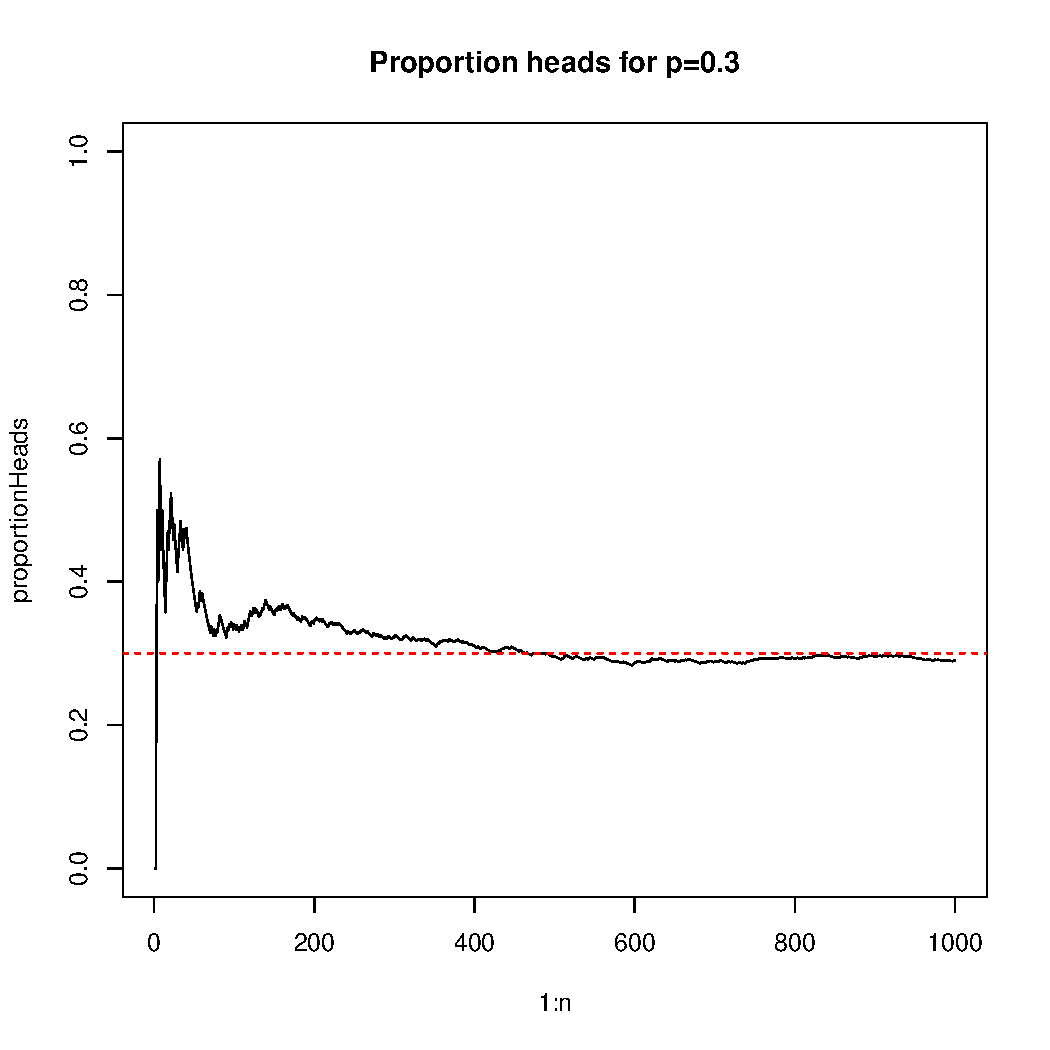
\includegraphics[width=0.6\textwidth]{ch1_2.21a.pdf}
\end{figure}


\newpage\noindent
Proportion of H vs T for $p=0.03$.
\begin{lstlisting}[style=RSyntax, title=R]
# 1.21 - Plotting proportion of H vs T
n = 5000
p = 0.03
coinTosses = sample(c("H","T"), prob = c(p, 1-p), size = n, replace = TRUE)
proportionHeads = rep(0, n)
headCount = 0
for(i in 1:n) {
    if (coinTosses[i] == "H") {
    headCount = headCount + 1
    } 
    proportionHeads[i] = headCount/i
} 

# PDF
pdf("~/ALLSTAT/ch1_2.21b.pdf")
plot(x = 1:n, y = proportionHeads, type = "l", ylim = c(0,1),
        main = paste0("Proportion heads for p=", p))
abline(h = p, col = "red", lty = "dashed")
dev.off()        
\end{lstlisting}

\medskip\noindent
\textbf{Result}\\
After some initial randomness due to few samples, we can see that the simulated results stabilizes
aroud 0.03, as expected. Did a simulation of 5000 to make the 'convergence' clearer. Note that the
y-axis only goes up to 0.1 in this plot.
\begin{figure}[H]
    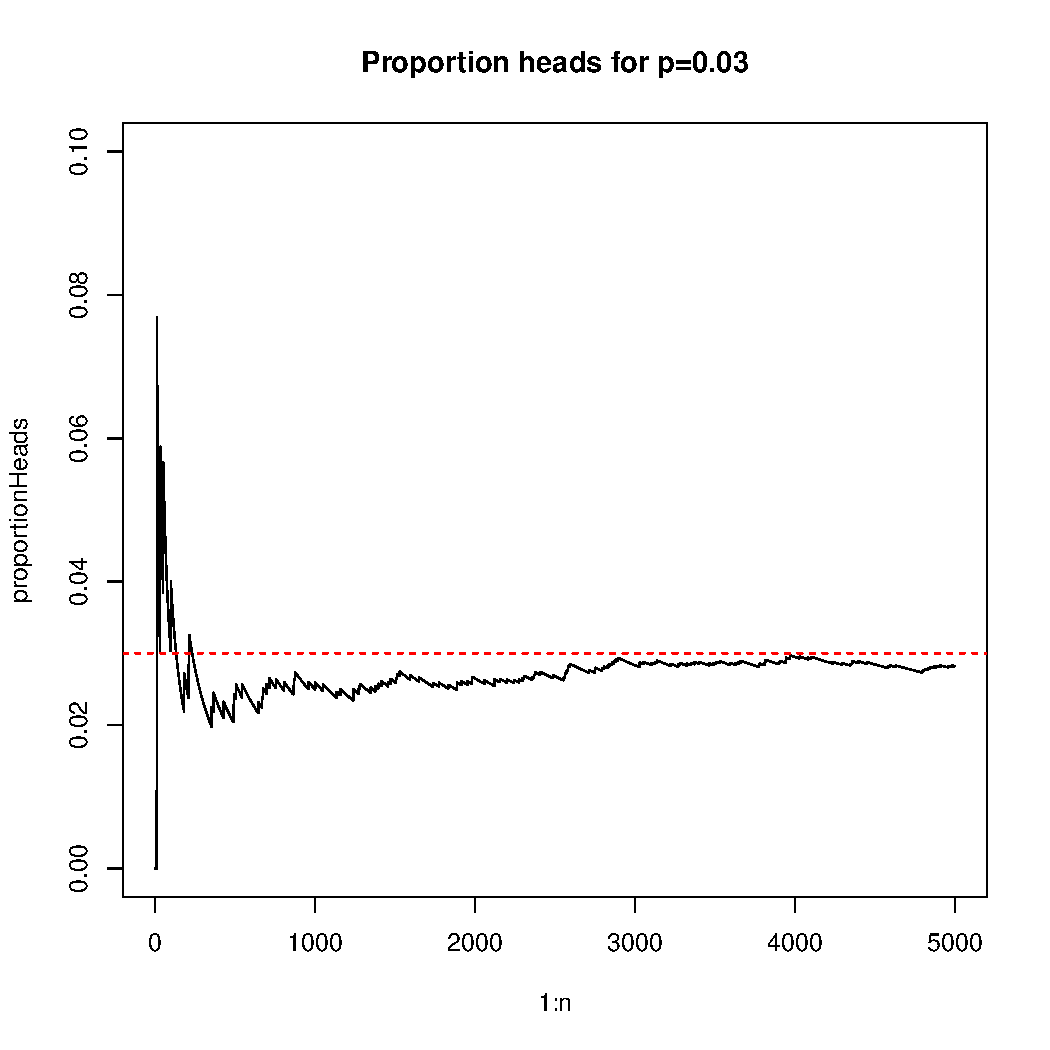
\includegraphics[width=0.6\textwidth]{ch1_2.21b.pdf}
\end{figure}



\newpage\noindent
\textbf{1.22}\\  % PDF page 16
Investigating some properties of Binomial random variables.
\begin{lstlisting}[style=RSyntax, title=R]
# 1.22 - Binomial Random Variables
REP = 10  # Number of simulations per n
p = 0.3   # Probability of H
sim10 = rep(0, REP)
sim100 = rep(0, REP)
sim1000 = rep(0, REP)
# Simulating 10
for(i in 1:REP) {
    # 1 means head
    coinTosses = sample(c(1,0), prob = c(p, 1-p), size = 10, replace = TRUE)
    sim10[i] = sum(coinTosses) 
} 
# Simulating 100
for(i in 1:REP) {
    # 1 means head
    coinTosses = sample(c(1,0), prob = c(p, 1-p), size = 100, replace = TRUE)
    sim100[i] = sum(coinTosses) 
} 
# Simulating 1000
for(i in 1:REP) {
    # 1 means head
    coinTosses = sample(c(1,0), prob = c(p, 1-p), size = 1000, replace = TRUE)
    sim1000[i] = sum(coinTosses) 
} 
df = data.frame(
    SIM10 = sim10,
    SIM100 = sim100,
    SIM1000 = sim1000
)       
# Output
df
apply(df, 2, mean)
\end{lstlisting}
As seen in the results, the mean of the 10 simulations is close to $np$ which would be 3, 30 and 300.
\begin{verbatim}
> df
    SIM10 SIM100 SIM1000
1     1     32     282
2     2     30     298
3     3     33     319
4     3     28     290
5     3     29     284
6     2     34     286
7     4     37     310
8     2     30     294
9     2     30     297
10    2     31     326
> apply(df, 2, mean)
    SIM10  SIM100 SIM1000 
    2.4    31.4   298.6 
\end{verbatim}



\newpage\noindent
\textbf{1.23}\\  % PDF page 17
Simulating conditional probabilities.
First we simulate an independent experiment.
\begin{lstlisting}[style=RSyntax, title=R]
# 1.23 - Simulating a fair die
options(digits=8)
numberOfTosses = 10000
A = c(2, 4, 6)
B = c(1, 2, 3, 4)
AandB = intersect(A, B) # c(2, 4)

dieTosses = sample(1:6, size = numberOfTosses, replace = TRUE)

# Calculating P(A), P(B), P(A)*P(B) and P(A cap B) 
PA = sum(dieTosses %in% A)/numberOfTosses
PB = sum(dieTosses %in% B)/numberOfTosses
PAandB = sum(dieTosses %in% AandB)/numberOfTosses

# Output
PA
PB
PA*PB
PAandB
\end{lstlisting}
Results from the calculation. As we can see, the estimates for $\P(A)\approx 1/2$ and
$\P(B)\approx 2/3$. Also $\P(A\cap B)\approx \P(A)\P(B) \approx 1/3$. Differences are probably due
to rounding errors.
\begin{verbatim}
> # Output
> PA
[1] 0.5005
> PB
[1] 0.6695
> PA*PB
[1] 0.33508475
> PAandB
[1] 0.3344
\end{verbatim}

\medskip\noindent
Now we will construct an experiment with a conditional probability. We will use a fair coin
and a die. When we get heads, this will correspond to 1 and the die is unchanged. If we get
tails, this will be 2 and will double the die count; so if we get tails and we roll a 2,
this will give us a 4.
$$
\begin{tabular}{c|cccccccccccc}
    \hline
    & 1 & 2 & 3 & 4 & 5 & 6 & 7 & 8 & 9 & 10 & 11 & 12 \\
    \hline
    $H$ & 1/12 & 1/12 & 1/12 & 1/12 & 1/12 & 1/12 & & & & & \\
    $T$ & & 1/12 & & 1/12& & 1/12& & 1/12& & 1/12& & 1/12 \\
    \hline
\end{tabular}
$$
Define the events: $A = \{2, 3, 4, 5, 6\}$ and $B = \{2, 4, 6, 8\}$ which will
give $A\cap B = \{2, 4, 6\}$. The theoretical probabilities are:
\begin{align*}
    \P(A) &= 8/12 = 2/3 = 0.666\\
    \P(B) &= 7/12 \approx 0.5833\\
    \P(A)\P(B) &= 7/18 \approx 0.3888\\
    \P(A\cap B) &= 1/2 = 0.5
\end{align*}


\newpage\noindent
Simulating conditional probabilities.
\begin{lstlisting}[style=RSyntax, title=R]
# 1.23 - Simulating a conditional probability
options(digits=8)
numberOfTosses = 10000
A = c(2, 3, 4, 5, 6)
B = c(2, 4, 6, 8)
AandB = intersect(A, B) # c(2, 4, 6)

dieTosses = sample(1:6, size = numberOfTosses, replace = TRUE)
coinTosses = sample(1:2, size = numberOfTosses, replace = TRUE)
jointToss = dieTosses*coinTosses

# Calculating P(A), P(B), P(A)*P(B) and P(A cap B)
PA = sum(jointToss %in% A)/numberOfTosses
PB = sum(jointToss %in% B)/numberOfTosses
PAandB = sum(jointToss %in% AandB)/numberOfTosses

# Output
PA
PB
PA*PB
PAandB    
\end{lstlisting}
\begin{verbatim}
> # Output
> PA
[1] 0.6691
> PB
[1] 0.5825
> PA*PB
[1] 0.38975075
> PAandB
[1] 0.4995
\end{verbatim}
Repeating the theoretical values from previous page:
\begin{align*}
    \P(A) &= 8/12 = 2/3 = 0.666\\
    \P(B) &= 7/12 \approx 0.5833\\
    \P(A)\P(B) &= 7/18 \approx 0.3888\\
    \P(A\cap B) &= 1/2 = 0.5
\end{align*}
The simulated results are very close to the theoretical calculations.
We can see that we do not have independence, as expected.







\begin{comment}

\bigskip\noindent
%%%%%%%%%%%%%%%%%%%%%%%%%%%%%%%%%%%%%%%%%%%%%%%%%%%%%%%%%%%%%%%%%%%%%%%%%%%%%%%
\textbf{1.X}\\  % PDF page 16


\begin{align*}
    A &= B
\end{align*}


\begin{equation*}
    A = B
    \tag*{\qed}
\end{equation*}


\end{comment}